\documentclass[12pt]{article}
\usepackage{hyperref}
\usepackage{listings}
\usepackage[margin=1in]{geometry}
\usepackage{enumitem}
\usepackage{multicol}
\usepackage{array}
\usepackage{titlesec}
\usepackage{helvet}
\renewcommand{\familydefault}{\sfdefault}
\usepackage{amsmath}     % For math equations
\usepackage{amssymb}     % For advanced math symbols
\usepackage{amsfonts} % For math fonts
\usepackage{gvv}
\usepackage{esint}
\usepackage[utf8]{inputenc}
\usepackage{graphicx}
\usepackage{pgfplots}
\pgfplotsset{compat=1.18}
\titleformat{\section}{\bfseries\large}{\thesection.}{1em}{}
\setlength{\parindent}{0pt}
\setlength{\parskip}{6pt}
\usepackage{multirow}

\usepackage{fancyhdr}     % For custom headers and footers

\pagestyle{fancy}         % Use the fancy page style
\fancyhf{}                % Clear existing header/footer

% Header customization
\renewcommand{\headrulewidth}{0.4pt}          % Horizontal line at top
\fancyhead[L]{\textbf{GATE 2018}}                       % Page number on left
\fancyhead[R]{\textbf{COMPUTER SCIENCE AND INFORMATION TECHNOLOGY}}  % Custom text on right
\cfoot{\thepage}

\usepackage[siunitx,RPvoltages]{circuitikz}
\usepackage{tikz}
\usepackage{float}
\usepackage{caption}

\begin{document}

\begin{center}
    {\Large \textbf{GA - GENERAL APTITUDE}}
\end{center}



\begin{enumerate}

\item[] \textbf{Q1 - Q5 carry one mark each.}

\item ``From where are they bringing their books? \_\_\_\_\_\_ bringing \_\_\_\_\_\_ books from \_\_\_\_\_\_.''

The words that best fill the blanks in the above sentence are
\begin{enumerate}
\item Their, they’re, there
\item They’re, their, there
\item There, their, they’re
\item They’re, there, there
\end{enumerate}

(GATE CS 2018)

\item ``A \_\_\_\_\_\_ investigation can sometimes yield new facts, but typically organized ones are more successful.''

The word that best fills the blank in the above sentence is
\begin{multicols}{4}
\begin{enumerate}
\item meandering
\item timely
\item consistent
\item systematic
\end{enumerate}
\end{multicols}

(GATE CS 2018)

\item The area of a square is $d$. What is the area of the circle which has the diagonal of the square as its diameter?

\begin{multicols}{4}
\begin{enumerate}
\item $\pi d$
\item $\pi d^2$
\item $\dfrac{1}{4}\pi d^2$
\item $\dfrac{1}{2}\pi d$
\end{enumerate}
\end{multicols}

(GATE CS 2018)

\item What would be the smallest natural number which when divided either by 20 or by 42 or by 76 leaves a remainder of 7 in each case?

\begin{multicols}{4}
\begin{enumerate}
\item 3047
\item 6047
\item 7987
\item 63847
\end{enumerate}
\end{multicols}

(GATE CS 2018)

\item What is the missing number in the following sequence?
$$
2,\;12,\;60,\;240,\;720,\;1440,\;\_\_\_\_\_\_,\;0
$$

\begin{multicols}{4}
\begin{enumerate}
\item 2880
\item 1440
\item 720
\item 0
\end{enumerate}
\end{multicols}

(GATE CS 2018)

\item[] \textbf{Q6 - Q10 carry two marks each.}

\item In appreciation of the social improvements completed in a town, a wealthy philanthropist decided to gift Rs $750$ to each male senior citizen in the town and Rs $1000$ to each female senior citizen. Altogether, there were $300$ senior citizens eligible for this gift. However, only $8/9$ of the eligible men and $2/3$ of the eligible women claimed the gift. How much money (in Rupees) did the philanthropist give away in total?

\begin{multicols}{2}
\begin{enumerate}
\item 1,50,000
\item 2,00,000
\item 1,75,000
\item 1,51,000
\end{enumerate}
\end{multicols}
(GATE CS 2018)

\item If $pqr \neq 0$ and 
$$p^{-x} = \frac{1}{q}, \quad q^{-y} = \frac{1}{r}, \quad r^{-z} = \frac{1}{p},$$ 
what is the value of the product $xyz$?

\begin{multicols}{4}
\begin{enumerate}
\item $-1$
\item $\dfrac{1}{pqr}$
\item $1$
\item $pqr$
\end{enumerate}
\end{multicols}
(GATE CS 2018)

\item In a party, $60\%$ of the invited guests are male and $40\%$ are female. If $80\%$ of the invited guests attended the party and if all the invited female guests attended, what would be the ratio of males to females among the attendees in the party?

\begin{multicols}{4}
\begin{enumerate}
\item 2:3
\item 1:1
\item 3:2
\item 2:1
\end{enumerate}
\end{multicols}
(GATE CS 2018)

\item In the figure below, $\angle DEC + \angle BFC$ is equal to $\_\_\_\_\_\_\_\_$.

\begin{figure}[H]
    \centering
    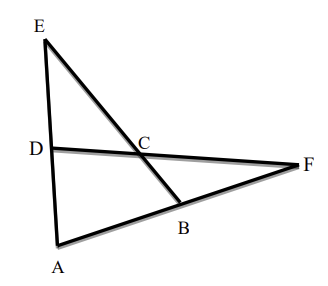
\includegraphics[width=0.5\columnwidth]{figs/ass6_0_q9.png}
    \caption{}
    \label{fig:placeholder}
\end{figure}

\begin{multicols}{2}
\begin{enumerate}
\item $\angle BCD - \angle BAD$
\item $\angle BAD + \angle BCF$
\item $\angle BAD + \angle BCD$
\item $\angle CBA + \angle ADC$
\end{enumerate}
\end{multicols}
(GATE CS 2018)

\item A six sided unbiased die with four green faces and two red faces is rolled seven times.
Which of the following combinations is the most likely outcome of the experiment?

\begin{enumerate}
\item Three green faces and four red faces.
\item Four green faces and three red faces.
\item Five green faces and two red faces.
\item Six green faces and one red face.
\end{enumerate}
(GATE CS 2018)


\end{enumerate}

\newpage

\begin{center}
    {\Large \textbf{COMPUTER SCIENCE AND TECHNOLOGY}}
\end{center}

\begin{enumerate}

\item[] \textbf{Q1 - Q25 carry one mark each.}

\item Which one of the following is a closed form expression for the generating function of the sequence $\{a_n\}$, where $a_n = 2n + 3$ for all $n = 0, 1, 2, \dots$?

\begin{multicols}{4}
\begin{enumerate}
\item $\dfrac{3}{(1-x)^2}$
\item $\dfrac{3x}{(1-x)^2}$
\item $\dfrac{2-x}{(1-x)^2}$
\item $\dfrac{3-x}{(1-x)^2}$
\end{enumerate}
\end{multicols}
(GATE CS 2018)

\item Consider the following C program.

\begin{verbatim}
#include<stdio.h>
struct Ournode{
   char x,y,z;
};

int main(){
   struct Ournode p = {'1','0','a'+2};
   struct Ournode *q = &p;
   printf("%c, %c", *((char*)q+1), *((char*)q+2));
   return 0;
}
\end{verbatim}

The output of this program is:

\begin{multicols}{4}
\begin{enumerate}
\item 0, c
\item 0, a+2
\item '0', 'a+2'
\item '0', 'c'
\end{enumerate}
\end{multicols}
(GATE CS 2018)

\item A queue is implemented using a non-circular singly linked list. The queue has a head pointer and a tail pointer, as shown in the figure. Let $n$ denote the number of nodes in the queue. Let \texttt{enqueue} be implemented by inserting a new node at the head, and \texttt{dequeue} be implemented by deletion of a node from the tail.

\begin{figure}[H]
    \centering
    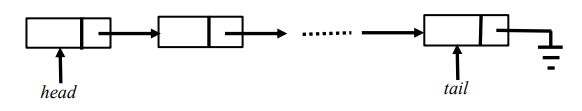
\includegraphics[width=0.5\columnwidth]{figs/ass6_a_q3.png}
    \caption{}
    \label{fig:placeholder}
\end{figure}

Which one of the following is the time complexity of the most time-efficient implementation of \texttt{enqueue} and \texttt{dequeue}, respectively, for this data structure?

\begin{multicols}{4}
\begin{enumerate}
\item $\theta(1), \theta(1)$
\item $\theta(1), \theta(n)$
\item $\theta(n), \theta(1)$
\item $\theta(n), \theta(n)$
\end{enumerate}
\end{multicols}
(GATE CS 2018)

\item Let $\oplus$ and $\odot$ denote the Exclusive OR and Exclusive NOR operations, respectively.  
Which one of the following is NOT CORRECT?

\begin{enumerate}
\item $P \oplus Q = \overline{P \odot Q}$
\item $\overline{P} \oplus Q = P \odot Q$
\item $\overline{P} \oplus \overline{Q} = P \odot Q$
\item $(P \oplus \overline{P}) \oplus Q = (P \odot \overline{P}) \odot \overline{Q}$
\end{enumerate}
(GATE CS 2018)

\item Consider the following processor design characteristics.  

I. Register-to-register arithmetic operations only  
II. Fixed-length instruction format  
III. Hardwired control unit  

Which of the characteristics above are used in the design of a RISC processor?

\begin{multicols}{4}
\begin{enumerate}
\item I and II only
\item II and III only
\item I and III only
\item I, II and III
\end{enumerate}
\end{multicols}
(GATE CS 2018)

\item Let $N$ be an NFA with $n$ states. Let $k$ be the number of states of a minimal DFA which is equivalent to $N$. Which one of the following is necessarily true?

\begin{multicols}{4}
\begin{enumerate}
\item $k \geq 2^n$
\item $k \geq n$
\item $k \leq n^2$
\item $k \leq 2^n$
\end{enumerate}
\end{multicols}
(GATE CS 2018)

\item The set of all recursively enumerable languages is

\begin{enumerate}
\item closed under complementation.
\item closed under intersection.
\item a subset of the set of all recursive languages.
\item an uncountable set.
\end{enumerate}
(GATE CS 2018)

\item Which one of the following statements is FALSE?

\begin{enumerate}
\item Context-free grammar can be used to specify both lexical and syntax rules.
\item Type checking is done before parsing.
\item High-level language programs can be translated to different Intermediate Representations.
\item Arguments to a function can be passed using the program stack.
\end{enumerate}
(GATE CS 2018)

\item The following are some events that occur after a device controller issues an interrupt while process $L$ is under execution.  

(P) The processor pushes the process status of $L$ onto the control stack.  
(Q) The processor finishes the execution of the current instruction.  
(R) The processor executes the interrupt service routine.  
(S) The processor pops the process status of $L$ from the control stack.  
(T) The processor loads the new PC value based on the interrupt.  

Which one of the following is the correct order in which the events above occur?

\begin{multicols}{4}
\begin{enumerate}
\item QPTRS
\item PTRSQ
\item TRPQS
\item QTPRS
\end{enumerate}
\end{multicols}
(GATE CS 2018)

\item Consider a process executing on an operating system that uses demand paging.  
The average time for a memory access in the system is $M$ units if the corresponding memory page is available in memory, and $D$ units if the memory access causes a page fault.  
It has been experimentally measured that the average time taken for a memory access in the process is $X$ units.  

Which one of the following is the correct expression for the page fault rate experienced by the process?

\begin{multicols}{2}
\begin{enumerate}
\item $\dfrac{(D - M)}{(X - M)}$
\item $\dfrac{(X - M)}{(D - M)}$
\item $\dfrac{(D - X)}{(D - M)}$
\item $\dfrac{(X - M)}{(D - X)}$
\end{enumerate}
\end{multicols}
(GATE CS 2018)

\item In an Entity-Relationship (ER) model, suppose $R$ is a many-to-one relationship from entity set $E1$ to entity set $E2$. Assume that $E1$ and $E2$ participate totally in $R$ and that the cardinality of $E1$ is greater than the cardinality of $E2$.  

Which one of the following is true about $R$?

\begin{enumerate}
\item Every entity in $E1$ is associated with exactly one entity in $E2$.
\item Some entity in $E1$ is associated with more than one entity in $E2$.
\item Every entity in $E2$ is associated with exactly one entity in $E1$.
\item Every entity in $E2$ is associated with at most one entity in $E1$.
\end{enumerate}
(GATE CS 2018)

\item Consider the following two tables and four queries in SQL.  

\textbf{Book} (\textit{isbn}, \textit{bname}), \quad \textbf{Stock} (\textit{isbn}, \textit{copies})

\textbf{Query 1:}
\begin{verbatim}
SELECT B.isbn, S.copies
FROM Book B INNER JOIN Stock S
ON B.isbn = S.isbn;
\end{verbatim}

\textbf{Query 2:}
\begin{verbatim}
SELECT B.isbn, S.copies
FROM Book B LEFT OUTER JOIN Stock S
ON B.isbn = S.isbn;
\end{verbatim}

\textbf{Query 3:}
\begin{verbatim}
SELECT B.isbn, S.copies
FROM Book B RIGHT OUTER JOIN Stock S
ON B.isbn = S.isbn;
\end{verbatim}

\textbf{Query 4:}
\begin{verbatim}
SELECT B.isbn, S.copies
FROM Book B FULL OUTER JOIN Stock S
ON B.isbn = S.isbn;
\end{verbatim}

Which one of the queries above is certain to have an output that is a superset of the outputs of the other three queries?

\begin{multicols}{4}
\begin{enumerate}
\item Query 1
\item Query 2
\item Query 3
\item Query 4
\end{enumerate}
\end{multicols}

(GATE CS 2018)

\item Match the following:

\begin{table}[!t]
\centering
\caption{} \label{}
\begin{tabular}{|l|l|}
\hline
\textbf{Field} & \textbf{Length in bits} \\ \hline
P. UDP Header’s Port Number & I. 48 \\ \hline
Q. Ethernet MAC Address & II. 8 \\ \hline
R. IPv6 Next Header & III. 32 \\ \hline
S. TCP Header’s Sequence Number & IV. 16 \\ \hline
\end{tabular}
\end{table}

\begin{multicols}{2}
\begin{enumerate}
\item P--III, Q--IV, R--II, S--I
\item P--II, Q--I, R--IV, S--III
\item P--IV, Q--I, R--II, S--III
\item P--IV, Q--I, R--III, S--II
\end{enumerate}
\end{multicols}

(GATE CS 2018)

\item Consider the following statements regarding the slow start phase of the TCP congestion control algorithm. Note that \textit{cwnd} stands for the TCP congestion window and \textit{MSS} denotes the Maximum Segment Size.

\noindent(i) The \textit{cwnd} increases by 2 MSS on every successful acknowledgment.\\
(ii) The \textit{cwnd} approximately doubles on every successful acknowledgement.\\
(iii) The \textit{cwnd} increases by 1 MSS every round trip time.\\
(iv) The \textit{cwnd} approximately doubles every round trip time.

\noindent Which one of the following is correct?

\begin{multicols}{2}
\begin{enumerate}
\item Only (i) and (iii) are true
\item Only (i) and (iii) are true
\item Only (iv) is true
\item Only (i) and (iv) are true
\end{enumerate}
\end{multicols}

(GATE CS 2018)

\item Two people, P and Q, decide to independently roll two identical dice, each with 6 faces, numbered 1 to 6. The person with the lower number wins. In case of a tie, they roll the dice repeatedly until there is no tie. Define a trial as a throw of the dice by P and Q. Assume that all 6 numbers on each dice are equi-probable and that all trials are independent. The probability (rounded to 3 decimal places) that one of them wins on the third trial is \_\_\_\_.

(GATE CS 2018)

\item The value of $ \displaystyle \int_{0}^{\pi/4} x \cos(x^2)\,dx $ correct to three decimal places (assuming that $ \pi = 3.14 $) is \_\_\_\_.

(GATE CS 2018)

\item Consider a matrix $A = u v^{T}$ where u=\myvec{1\\2},\ v=\myvec{1\\1}. Note that $v^{T}$ denotes the transpose of $v$. The largest eigenvalue of $A$ is \_\_\_\_.

(GATE CS 2018)

\item The chromatic number of the following graph is \_\_\_\_. 

\begin{figure}[H]
    \centering
    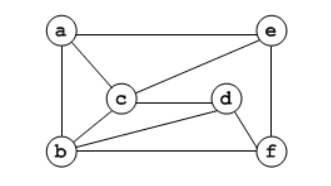
\includegraphics[width=0.5\columnwidth]{figs/ass6_a_q18.png}
    \caption{}
    \label{fig:placeholder}
\end{figure}

(GATE CS 2018)

\item Let $G$ be a finite group on 84 elements. The size of a largest possible proper subgroup of $G$ is \_\_\_\_\_\_.  

(GATE CS 2018)

\item The postorder traversal of a binary tree is $8,9,6,7,4,5,2,3,1$. The inorder traversal of the same tree is $8,6,9,4,7,2,5,1,3$. The height of a tree is the length of the longest path from the root to any leaf. The height of the binary tree above is \_\_\_\_\_\_.  

(GATE CS 2018)

\item Consider the following C program:
\begin{verbatim}
#include <stdio.h>

int counter = 0;

int calc (int a, int b) {
    int c;
    counter++;
    if (b==3) return (a*a+a);
    else {
        c = calc(a, b/3);
        return (c*c+c);
    }
}

int main() {
    calc(4, 81);
    printf("%d", counter);
    return 0;
}
\end{verbatim}

The output of this program is \_\_\_\_\_\_.  

(GATE CS 2018)

\item Consider the sequential circuit shown in the figure, where both flip-flops used are positive edge-triggered D flip-flops.  

\begin{figure}[H]
    \centering
    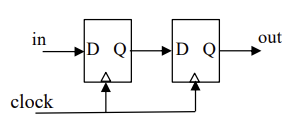
\includegraphics[width=0.5\columnwidth]{figs/ass6_a_q22.png}
    \caption{}
    \label{fig:placeholder}
\end{figure}

The number of states in the state transition diagram of this circuit that have a transition back to the same state on some value of “in” is \_\_\_\_\_\_.  

(GATE CS 2018)

\item A 32-bit wide main memory unit with a capacity of 1 GB is built using $256M \times 4$-bit DRAM chips. The number of rows of memory cells in the DRAM chip is $2^{14}$. The time taken to perform one refresh operation is 50 nanoseconds. The refresh period is 2 milliseconds. The percentage (rounded to the closest integer) of the time available for performing the memory read/write operations in the main memory unit is \_\_\_\_\_\_.  

(GATE CS 2018)

\item Consider a system with 3 processes that share 4 instances of the same resource type. Each process can request a maximum of $K$ instances. Resource instances can be requested and released only one at a time. The largest value of $K$ that will always avoid deadlock is \_\_\_\_\_\_.  

(GATE CS 2018)

\item Consider a long-lived TCP session with an end-to-end bandwidth of 1 Gbps ($= 10^{9}$ bits-per-second). The session starts with a sequence number of 1234. The minimum time (in seconds, rounded to the closest integer) before this sequence number can be used again is \_\_\_\_\_\_.  

(GATE CS 2018)



\item[] \textbf{Q26 - Q55 carry two marks each.}


\item Consider a matrix $P$ whose only eigenvectors are the multiples of \myvec{ 1 \\ 4 }.

Consider the following statements.  
(I) $P$ does not have an inverse  
(II) $P$ has a repeated eigenvalue  
(III) $P$ cannot be diagonalized  

Which one of the following options is correct?

\begin{multicols}{2}
\begin{enumerate}
\item Only I and III are necessarily true
\item Only II is necessarily true
\item Only I and II are necessarily true
\item Only II and III are necessarily true
\end{enumerate}
\end{multicols}

(GATE CS 2018)

\item Let $N$ be the set of natural numbers. Consider the following sets.  

P: Set of Rational numbers (positive and negative)  
Q: Set of functions from $\{0,1\}$ to $N$  
R: Set of functions from $N$ to $\{0,1\}$  
S: Set of finite subsets of $N$  

Which of the sets above are countable?  

\begin{multicols}{4}
\begin{enumerate}
\item Q and S only
\item P and S only
\item P and R only
\item P, Q and S only
\end{enumerate}
\end{multicols}

(GATE CS 2018)

\item Consider the first-order logic sentence  

$$
\varphi \equiv \exists s \exists t \exists u \forall v \forall w \forall x \forall y \; \psi(s,t,u,v,w,x,y)
$$  

where $\psi(s,t,u,v,w,x,y)$ is a quantifier-free first-order logic formula using only predicate symbols, and possibly equality, but no function symbols. Suppose $\varphi$ has a model with a universe containing 7 elements.  

Which one of the following statements is necessarily true?  

\begin{enumerate}
\item There exists at least one model of $\varphi$ with universe of size less than or equal to 3.
\item There exists no model of $\varphi$ with universe of size less than or equal to 3.
\item There exists no model of $\varphi$ with universe of size greater than 7.
\item Every model of $\varphi$ has a universe of size equal to 7.
\end{enumerate}

(GATE CS 2018)

\item Consider the following C program:

\begin{verbatim}
#include<stdio.h>

void fun1(char *s1, char *s2){
    char *tmp;
    tmp = s1;
    s1 = s2;
    s2 = tmp;
}

void fun2(char **s1, char **s2){
    char *tmp;
    tmp = *s1;
    *s1 = *s2;
    *s2 = tmp;
}

int main(){
    char *str1 = "Hi", *str2 = "Bye";
    fun1(str1, str2);   printf("%s %s ", str1, str2);
    fun2(&str1, &str2); printf("%s %s", str1, str2);
    return 0;
}
\end{verbatim}

The output of the program above is

\begin{multicols}{2}
\begin{enumerate}
\item Hi Bye Bye Hi
\item Hi Bye Hi Bye
\item Bye Hi Hi Bye
\item Bye Hi Bye Hi
\end{enumerate}
\end{multicols}

(GATE CS 2018)

\item Let $G$ be a simple undirected graph. Let $T_D$ be a depth first search tree of $G$. Let $T_B$ be a breadth first search tree of $G$. Consider the following statements:

\begin{enumerate}
\item[(I)] No edge of $G$ is a cross edge with respect to $T_D$. (A cross edge in $G$ is between two nodes neither of which is an ancestor of the other in $T_D$.)
\item[(II)] For every edge $(u,v)$ of $G$, if $u$ is at depth $i$ and $v$ is at depth $j$ in $T_B$, then $|i-j| = 1$.
\end{enumerate}

Which of the statements above must necessarily be true?

\begin{multicols}{2}
\begin{enumerate}
\item I only
\item II only
\item Both I and II
\item Neither I nor II
\end{enumerate}
\end{multicols}

(GATE CS 2018)

\item Assume that multiplying a matrix $G_1$ of dimension $p\times q$ with another matrix $G_2$ of dimension $q\times r$ requires $pqr$ scalar multiplications. Computing the product of $n$ matrices $G_1G_2G_3\ldots G_n$ can be done by parenthesizing in different ways. Define $G_iG_{i+1}$ as an explicitly computed pair for a given parenthesization if they are directly multiplied. For example, in the matrix multiplication chain $G_1G_2G_3G_4G_5G_6$ using parenthesization $(G_1(G_2G_3))(G_4(G_5G_6))$, $G_2G_3$ and $G_5G_6$ are the only explicitly computed pairs.

Consider a matrix multiplication chain $F_1F_2F_3F_4F_5$, where matrices $F_1, F_2, F_3, F_4$ and $F_5$ are of dimensions $2\times 25$, $25\times 3$, $3\times 16$, $16\times 1$ and $1\times 1000$, respectively. In the parenthesization of $F_1F_2F_3F_4F_5$ that minimizes the total number of scalar multiplications, the explicitly computed pairs is/are
\begin{multicols}{2}
\begin{enumerate}
\item $F_1F_2$ and $F_3F_4$ only
\item $F_2F_3$ only
\item $F_3F_4$ only
\item $F_1F_2$ and $F_4F_5$ only
\end{enumerate}
\end{multicols}
(GATE CS 2018)

\item Consider the following C code. Assume that \texttt{unsigned long int} type length is 64 bits.

\begin{verbatim}
unsigned long int fun(unsigned long int n){
    unsigned long int i, j = 0, sum = 0;
    for (i = n; i > 1; i = i/2) j++;
    for (; j > 1; j = j/2) sum++;
    return(sum);
}
\end{verbatim}

The value returned when we call \texttt{fun} with the input $2^{40}$ is
\begin{multicols}{4}
\begin{enumerate}
\item 4
\item 5
\item 6
\item 40
\end{enumerate}
\end{multicols}
(GATE CS 2018)

\item Consider the unsigned 8-bit fixed point binary number representation below,
$$
\underbrace{b_7\;b_6\;b_5\;b_4\;b_3}_{\text{integer part}},\underbrace{b_2\;b_1\;b_0}_{\text{fractional part}}
$$
where the position of the binary point is between $b_3$ and $b_2$. Assume $b_7$ is the most significant bit. Some of the decimal numbers listed below cannot be represented exactly in the above representation:
$$
\text{(i) }31.500 \quad \text{(ii) }0.875 \quad \text{(iii) }12.100 \quad \text{(iv) }3.001
$$
Which one of the following statements is true?
\begin{enumerate}
\item None of (i), (ii), (iii), (iv) can be exactly represented
\item Only (ii) cannot be exactly represented
\item Only (iii) and (iv) cannot be exactly represented
\item Only (i) and (ii) cannot be exactly represented
\end{enumerate}
(GATE CS 2018)

\item The size of the physical address space of a processor is $2^P$ bytes. The word length is $2^W$ bytes. The capacity of cache memory is $2^N$ bytes. The size of each cache block is $2^M$ words. For a $K$-way set-associative cache memory, the length (in number of bits) of the tag field is
\begin{multicols}{2}
\begin{enumerate}
\item $P - N - \log_2 K$
\item $P - N + \log_2 K$
\item $P - N - M - W - \log_2 K$
\item $P - N - M - W + \log_2 K$
\end{enumerate}
\end{multicols}
(GATE CS 2018)

\item Consider the following languages:

I.\ $\{a^m b^n c^p d^q \mid m+p = n+q,\ \text{where } m,n,p,q \ge 0\}$

II.\ $\{a^m b^n c^p d^q \mid m = n \text{ and } p = q,\ \text{where } m,n,p,q \ge 0\}$

III.\ $\{a^m b^n c^p d^q \mid m = n \text{ and } p \ne q,\ \text{where } m,n,p,q \ge 0\}$

IV.\ $\{a^m b^n c^p d^q \mid mn = p + q,\ \text{where } m,n,p,q \ge 0\}$

Which of the languages above are context-free?
\begin{multicols}{2}
\begin{enumerate}
\item I and IV only
\item I and II only
\item II and III only
\item II and IV only
\end{enumerate}
\end{multicols}
(GATE CS 2018)

\item Consider the following problems. $L(G)$ denotes the language generated by a grammar $G$. $L(M)$ denotes the language accepted by a machine $M$.

(i) For an unrestricted grammar $G$ and a string $w$, whether $w \in L(G)$

(ii) Given a Turing machine $M$, whether $L(M)$ is regular

(iii) Given two grammars $G_1$ and $G_2$, whether $L(G_1)=L(G_2)$

(iv) Given an NFA $N$, whether there is a deterministic PDA $P$ such that $N$ and $P$ accept the same language.

Which one of the following statements is correct?
\begin{multicols}{2}
\begin{enumerate}
\item Only I and II are undecidable
\item Only III is undecidable
\item Only II and IV are undecidable
\item Only I, II and III are undecidable
\end{enumerate}
\end{multicols}
(GATE CS 2018)

\item A lexical analyzer uses the following patterns to recognize three tokens $T_1$, $T_2$, and $T_3$ over the alphabet $\{a,b,c\}$.

\begin{align}
T_1 &: \ a?(b|c)^*a\\
T_2 &: \ b?(a|c)^*b\\
T_3 &: \ c?(b|a)^*c
\end{align}

Note that “$x?$” means $0$ or $1$ occurrence of the symbol $x$. Note also that the analyzer outputs the token that matches the longest possible prefix.

If the string \texttt{bbaaacabc} is processed by the analyzer, which one of the following is the sequence of tokens it outputs?
\begin{multicols}{4}
\begin{enumerate}
\item $T_1T_2T_3$
\item $T_1T_1T_3$
\item $T_2T_1T_3$
\item $T_3T_3$
\end{enumerate}
\end{multicols}
(GATE CS 2018)

\item Consider the following parse tree for the expression $a \# b \$ c \$ d \# e \# f$, involving two binary operators \$ and \#.
\emph{(Parse tree as shown in the question.)}

\begin{figure}[H]
    \centering
    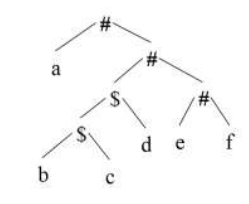
\includegraphics[width=0.5\columnwidth]{figs/ass6_a_q38.png}
    \caption{}
    \label{fig:placeholder}
\end{figure}

Which one of the following is correct for the given parse tree?
\begin{enumerate}
\item \$ has higher precedence and is left associative; \# is right associative
\item \# has higher precedence and is left associative; \$ is right associative
\item \$ has higher precedence and is left associative; \# is left associative
\item \# has higher precedence and is right associative; \$ is left associative
\end{enumerate}
(GATE CS 2018)

\item In a system, there are three types of resources: $E$, $F$ and $G$. Four processes $P_{0}, P_{1}, P_{2}$ and $P_{3}$
execute concurrently. At the outset, the processes have declared their maximum resource
requirements using a matrix named \texttt{Max} as given below. For example, $\texttt{Max}[P_2,F]$ is the
maximum number of instances of $F$ that $P_2$ would require. The number of instances of the
resources allocated to the various processes at any given state is given by a matrix named
\texttt{Allocation}.

Consider a state of the system with the \texttt{Allocation} matrix as shown below, and in which
\textbf{3 instances of $E$ and 3 instances of $F$ are the only resources available}.

\begin{table}[H]
\centering
\caption{} \label{}
\begin{tabular}{c c}
\begin{tabular}{|c|ccc|}
\multicolumn{4}{c}{\textbf{Allocation}}\\
\hline
     & $E$ & $F$ & $G$\\ \hline
$P_0$& 1 & 0 & 1\\
$P_1$& 1 & 1 & 2\\
$P_2$& 1 & 0 & 3\\
$P_3$& 2 & 0 & 0\\
\hline
\end{tabular}
&
\begin{tabular}{|c|ccc|}
\multicolumn{4}{c}{\textbf{Max}}\\
\hline
     & $E$ & $F$ & $G$\\ \hline
$P_0$& 4 & 3 & 1\\
$P_1$& 2 & 1 & 4\\
$P_2$& 3 & 1 & 3\\
$P_3$& 5 & 4 & 1\\
\hline
\end{tabular}
\end{tabular}
\end{table}

From the perspective of deadlock avoidance, which one of the following is true?

\begin{enumerate}
\item The system is in \textit{safe} state.
\item The system is not in \textit{safe} state, but would be \textit{safe} if one more instance of $E$ were available
\item The system is not in \textit{safe} state, but would be \textit{safe} if one more instance of $F$ were available
\item The system is not in \textit{safe} state, but would be \textit{safe} if one more instance of $G$ were available
\end{enumerate}

(GATE CS 2018)

\item Consider the following solution to the producer–consumer synchronization problem. The
shared buffer size is $N$. Three semaphores \texttt{empty}, \texttt{full} and \texttt{mutex} are defined with respective
initial values of $0$, $N$ and $1$. Semaphore \texttt{empty} denotes the number of available slots in the
buffer, for the consumer to read from. Semaphore \texttt{full} denotes the number of available slots
in the buffer, for the producer to write to. The placeholder variables, denoted by $P$, $Q$, $R$,
and $S$, in the code below can be assigned either \texttt{empty} or \texttt{full}. The valid semaphore
operations are: \texttt{wait()} and \texttt{signal()}.

\begin{table}[H]
\centering
\caption{} \label{}
\begin{tabular}{|p{0.45\linewidth}|p{0.45\linewidth}|}
\hline
\textbf{Producer:} &
\textbf{Consumer:} \\
\hline
\ttfamily
do\{ & do\{\\
\quad wait(P); & \quad wait(R);\\
\quad wait(mutex); & \quad wait(mutex);\\
\quad // Add item to buffer & \quad // Consume item from buffer\\
\quad signal(mutex); & \quad signal(mutex);\\
\quad signal(Q); & \quad signal(S);\\
\} while(1); &  \} while(1);\\

\hline
\end{tabular}
\end{table}

Which one of the following assignments to $P,\ Q,\ R$ and $S$ will yield the correct solution?

\begin{enumerate}
\item $P$: \texttt{full}, \quad $Q$: \texttt{full}, \quad $R$: \texttt{empty}, \quad $S$: \texttt{empty}
\item $P$: \texttt{empty}, \quad $Q$: \texttt{empty}, \quad $R$: \texttt{full}, \quad $S$: \texttt{full}
\item $P$: \texttt{full}, \quad $Q$: \texttt{empty}, \quad $R$: \texttt{empty}, \quad $S$: \texttt{full}
\item $P$: \texttt{empty}, \quad $Q$: \texttt{full}, \quad $R$: \texttt{full}, \quad $S$: \texttt{empty}
\end{enumerate}


(GATE CS 2018)

\item Consider the relations $r(A,B)$ and $s(B,C)$, where $s.B$ is a primary key and $r.B$ is a foreign
key referencing $s.B$. Consider the query
$$
Q:\quad r \Join \bigl(\sigma_{B \le 5}(s)\bigr)
$$
Let \texttt{LOJ} denote the natural left outer-join operation. Assume that $r$ and $s$ contain no null
values.

Which one of the following queries is \textbf{NOT} equivalent to $Q$?

\begin{multicols}{2}
\begin{enumerate}
\item $\sigma_{B<5}\bigl(r \Join s\bigr)$
\item $\sigma_{B \le 5}\bigl(r \ \texttt{LOJ}\ s\bigr)$
\item $r \ \texttt{LOJ}\ \bigl(\sigma_{B \le 5}(s)\bigr)$
\item $\sigma_{B \le 5}(r)\ \texttt{LOJ}\ s$
\end{enumerate}
\end{multicols}

(GATE CS 2018)

\item Consider the following four relational schemas. For each schema, all non-trivial functional
dependencies are listed. The \underline{underlined} attributes are the respective primary keys.

\textbf{Schema I:} \emph{Registration (\underline{rollno}, courses)}\\
Field \texttt{courses} is a set-valued attribute containing the set of courses a student has
registered for.\\
Non-trivial functional dependency: \\
$\qquad \textit{rollno} \rightarrow \textit{courses}$

\textbf{Schema II:} \emph{Registration (\underline{rollno}, \underline{courseid}, email)}\\
Non-trivial functional dependencies: \\
$\qquad (\textit{rollno}, \textit{courseid}) \rightarrow \textit{email}$\\
$\qquad \textit{email} \rightarrow \textit{rollno}$

\textbf{Schema III:} \emph{Registration (\underline{rollno}, \underline{courseid}, marks, grade)}\\
Non-trivial functional dependencies: \\
$\qquad (\textit{rollno}, \textit{courseid}) \rightarrow \textit{marks}, \textit{grade}$\\
$\qquad \textit{marks} \rightarrow \textit{grade}$

\textbf{Schema IV:} \emph{Registration (\underline{rollno}, \underline{courseid}, credit)}\\
Non-trivial functional dependencies: \\
$\qquad (\textit{rollno}, \textit{courseid}) \rightarrow \textit{credit}$\\
$\qquad \textit{courseid} \rightarrow \textit{credit}$

Which one of the relational schemas above is in 3NF but not in BCNF?

\begin{multicols}{4}
\begin{enumerate}
\item Schema I
\item Schema II
\item Schema III
\item Schema IV
\end{enumerate}
\end{multicols}

(GATE CS 2018)

\item Let $G$ be a graph with $100!$ vertices, with each vertex labelled by a distinct permutation of
the numbers $1,2,\dots,100$. There is an edge between vertices $u$ and $v$ if and only if the label
of $u$ can be obtained by swapping two adjacent numbers in the label of $v$. Let $y$ denote the
degree of a vertex in $G$, and $z$ denote the number of connected components in $G$. Then,
$y + 10z = \_\_\_\_\_\_\_$.

(GATE CS 2018)

\item Consider Guwahati (G) and Delhi (D) whose temperatures can be classified as high (H),
medium (M) and low (L). Let $P(H_G)$ denote the probability that Guwahati has high
temperature. Similarly, $P(M_G)$ and $P(L_G)$ denote the probability of Guwahati having
medium and low temperatures respectively. Similarly, we use $P(H_D)$, $P(M_D)$ and $P(L_D)$ for
Delhi.

The following table gives the conditional probabilities for Delhi’s temperature given
Guwahati’s temperature.

\begin{table}[H]
\centering
\caption{} \label{} 
\begin{tabular}{|c|c|c|c|}
\hline
 & $H_D$ & $M_D$ & $L_D$ \\
\hline
$H_G$ & 0.40 & 0.48 & 0.12 \\
$M_G$ & 0.10 & 0.65 & 0.25 \\
$L_G$ & 0.01 & 0.50 & 0.49 \\
\hline
\end{tabular}
\end{table}

Consider the first row in the table above. The first entry denotes that if Guwahati has high
temperature ($H_G$) then the probability of Delhi also having a high temperature ($H_D$) is 0.40;
i.e., $P(H_D|H_G)=0.40$. Similarly, the next two entries are $P(M_D|H_G)=0.48$ and
$P(L_D|H_G)=0.12$. Similarly for the other rows.

If it is known that $P(H_G)=0.2$, $P(M_G)=0.5$, and $P(L_G)=0.3$, then the probability
(correct to two decimal places) that Guwahati has high temperature given that Delhi has high
temperature is \_\_\_\_\_\_\_.

(GATE CS 2018)

\item Consider the following program written in pseudo-code. Assume that $x$ and $y$ are integers.

\begin{verbatim}
Count(x,y) {
    if (y != 1) {
        if (x != 1) {
            print("*");
            Count(x/2, y);
        }
        else {
            y = y-1;
            Count(1024, y);
        }
    }
}
\end{verbatim}

The number of times that the \texttt{print} statement is executed by the call
\texttt{Count(1024,1024)} is \_\_\_\_\_\_\_.

(GATE CS 2018)

\item The number of possible min-heaps containing each value from
$\{1,2,3,4,5,6,7\}$ exactly once is \_\_\_\_\_\_\_.

(GATE CS 2018)

\item Consider the following undirected graph $G$:

\begin{figure}[H]
    \centering
    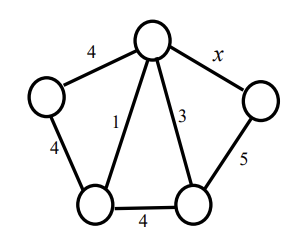
\includegraphics[width=0.5\columnwidth]{figs/ass6_a_q47.png}
    \caption{}
    \label{fig:placeholder}
\end{figure}
\textit{(diagram omitted; edge weights as shown with one edge of weight $x$)}\\[2pt]
Choose a value for $x$ that will maximize the number of minimum weight spanning trees (MWSTs) of $G$. The number of MWSTs of $G$ for this value of $x$ is \_\_\_\_\_\_\_.\\
(GATE CS 2018)

\item Consider the weights and values of items listed below. Note that there is only one unit of each item.

\begin{table}[H]
\centering
\caption{} \label{} 
\begin{tabular}{|c|c|c|}
\hline
\textbf{Item number} & \textbf{Weight (in Kgs)} & \textbf{Value (in Rupees)}\\
\hline
1 & 10 & 60\\
2 & 7 & 28\\
3 & 4 & 20\\
4 & 2 & 24\\
\hline
\end{tabular}
\end{table}

The task is to pick a subset of these items such that their total weight is no more than $11$ Kgs and their total value is maximized. Moreover, no item may be split. The total value of items picked by an optimal algorithm is denoted by $V_{\text{opt}}$. A greedy algorithm sorts the items by their value-to-weight ratios in descending order and packs them greedily, starting from the first item in the ordered list. The total value of items picked by the greedy algorithm is denoted by $V_{\text{greedy}}$.

The value of $V_{\text{opt}}-V_{\text{greedy}}$ is \_\_\_\_\_\_\_.\\
(GATE CS 2018)

\item Consider the minterm list form of a Boolean function $F$ given below.
$$
F(P,Q,R,S)=\sum m(0,2,5,7,9,11)+d(3,8,10,12,14)
$$
Here, $m$ denotes a minterm and $d$ denotes a don’t care term. The number of essential prime implicants of the function $F$ is \_\_\_\_\_\_\_.\\
(GATE CS 2018)

\item The instruction pipeline of a RISC processor has the following stages: Instruction Fetch (IF), Instruction Decode (ID), Operand Fetch (OF), Perform Operation (PO) and Writeback (WB). The IF, ID, OF and WB stages take $1$ clock cycle each for every instruction. Consider a sequence of $100$ instructions. In the PO stage, $40$ instructions take $3$ clock cycles each, $35$ instructions take $2$ clock cycles each, and the remaining $25$ instructions take $1$ clock cycle each. Assume that there are no data hazards and no control hazards.

The number of clock cycles required for completion of execution of the sequence of instructions is \_\_\_\_\_\_\_.

(GATE CS 2018)

\item A processor has $16$ integer registers $(\mathrm{R0}, \mathrm{R1},\ldots,\mathrm{R15})$ and $64$ floating point registers $(\mathrm{F0},\ldots,\mathrm{F63})$. It uses a $2$-byte instruction format. There are four categories of instructions: Type-1, Type-2, Type-3, and Type-4. Type-1 category consists of four instructions, each with three integer register operands (3Rs). Type-2 category consists of eight instructions, each with two floating point register operands (2Fs). Type-3 category consists of fourteen instructions, each with one integer register operand and one floating point register operand (1R+1F). Type-4 category consists of $N$ instructions, each with a floating point register operand (1F).

The maximum value of $N$ is \_\_\_\_\_\_\_.

(GATE CS 2018)

\item Given a language $L$, define $L^i$ as follows:
$$
L^0=\{\varepsilon\},\qquad L^i=L^{\,i-1}\cdot L\ \text{ for all } i>0.
$$
The \emph{order} of a language $L$ is defined as the smallest $k$ such that $L^k=L^{k+1}$. Consider the language $L_1$ (over alphabet $\{0\}$) accepted by the automaton shown below.

\begin{figure}[H]
    \centering
    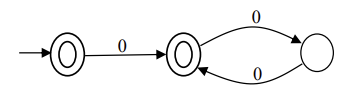
\includegraphics[width=0.5\columnwidth]{figs/ass6_a_q52.png}
    \caption{}
    \label{fig:placeholder}
\end{figure}

The order of $L_1$ is \_\_\_\_\_\_\_.

(GATE CS 2018)


\item Consider a storage disk with $4$ platters (numbered as $0,1,2,3$), $200$ cylinders (numbered as $0,1,\ldots,199$), and $256$ sectors per track (numbered as $0,1,\ldots,255$). The following $6$ disk requests of the form [sector number, cylinder number, platter number] are received by the disk controller at the same time:  

$$
[120,72,2],\ [180,134,1],\ [60,20,0],\ [212,86,3],\ [56,116,2],\ [118,16,1]
$$

Currently the head is positioned at sector number $100$ of cylinder $80$, and is moving towards higher cylinder numbers. The average power dissipation in moving the head over $100$ cylinders is $20$ milliwatts and for reversing the direction of the head movement once is $15$ milliwatts. Power dissipation associated with rotational latency and switching of head between different platters is negligible.  

The total power consumption in milliwatts to satisfy all of the above disk requests using the Shortest Seek Time First disk scheduling algorithm is \_\_\_\_\_\_\_.  

(GATE CS 2018)

\item Consider an IP packet with a length of $4500$ bytes that includes a $20$-byte IPv4 header and a $40$-byte TCP header. The packet is forwarded to an IPv4 router that supports a Maximum Transmission Unit (MTU) of $600$ bytes. Assume that the length of the IP header in all the outgoing fragments of this packet is $20$ bytes. Assume that the fragmentation offset value stored in the first fragment is $0$.  

The fragmentation offset value stored in the third fragment is \_\_\_\_\_\_\_.  

(GATE CS 2018)

\item Consider a simple communication system where multiple nodes are connected by a shared broadcast medium (like Ethernet or wireless). The nodes in the system use the following carrier-sense based medium access protocol. A node that receives a packet to transmit will carrier-sense the medium for $5$ units of time. If the node does not detect any other transmission in this duration, it starts transmitting its packet in the next time unit. If the node detects another transmission, it waits until this other transmission finishes, and then begins to carrier-sense for $5$ time units again. Once they start to transmit, nodes do not perform any collision detection and continue transmission even if a collision occurs. All transmissions last for $20$ units of time. Assume that the transmission signal travels at the speed of $10$ meters per unit time in the medium.  

Assume that the system has two nodes $P$ and $Q$, located at a distance $d$ meters from each other. $P$ starts transmitting a packet at time $t=0$ after successfully completing its carrier-sense phase. Node $Q$ has a packet to transmit at time $t=0$ and begins to carrier-sense the medium.  

The maximum distance $d$ (in meters, rounded to the closest integer) that allows $Q$ to successfully avoid a collision between its proposed transmission and $P$’s ongoing transmission is \_\_\_\_\_\_\_.  

(GATE CS 2018)

\end{enumerate}

\begin{center}
    {\Large \textbf{END OF THE QUESTION PAPER}}
\end{center}

\end{document}
